\section{Diagrama de Banco de Dados}

\subsection{Modelo Entidade-Relacionamento (MER)}

O Modelo Entidade-Relacionamento (MER)~\cite{chen1976} foi utilizado para representar a estrutura conceitual do banco de dados da plataforma de verificação do teste do iodo. O objetivo desse modelo é demonstrar as entidades presentes no sistema, seus atributos e os relacionamentos existentes entre elas.

\begin{figure}[H]
\centering
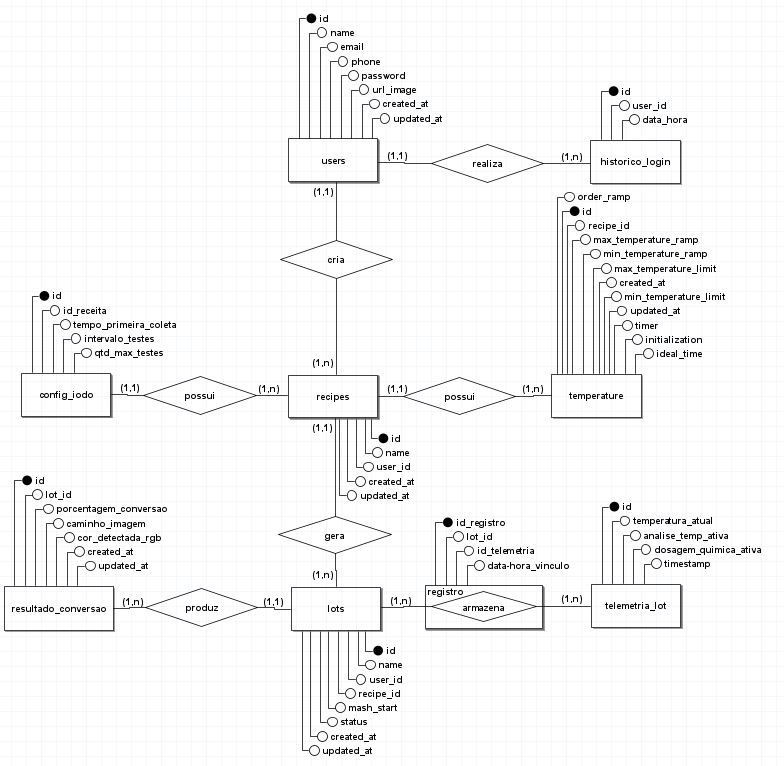
\includegraphics[width=0.9\linewidth]{imgs/diagrama-mer.png}
\caption{Modelo Entidade-Relacionamento}
\label{fig:diagrama-de-banco-de-dados}
\end{figure}